\subsection{Weather station}\label{sec:weather_station}
One of the devices that is connected to the ODROID is the Lufft WS503-UMB weather station \cite{weatherstation_registers}. It is connected to an adapter that converts the Modbus RTU connection to an USB that can be connected to the ODROID (See \Cref{fig:weather_station_connection}). This station is capable of measuring air pressure, relative humidity, solar radiation, air pressure, wind direction and wind speed. The data that this weather station processes is collected \ref{eis:1.1} and used to display local weather information to both the user \ref{eis:1.6} and the administrator. It could also be used to add functionality, such as disabling charging when the outside temperature is too low \cite{battery_temperature} or checking if the solar panels are functioning by comparing output power to solar radiation.\\

\begin{figure}[!ht]
  \centering
    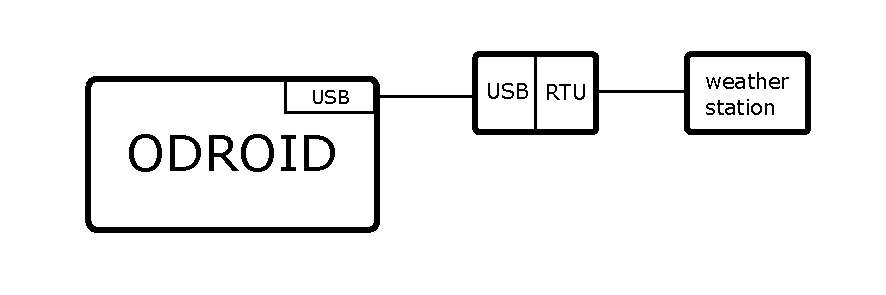
\includegraphics[width=0.6\textwidth]{images/ODROID_weather_station.pdf}
      \caption{The connection of the weather station}\label{fig:weather_station_connection}
\end{figure}

The polling of the weather stations registers is set to roughly every 15 seconds. Although the maximum polling rate \ref{eis:3.2} is technically possible of going down to 10 seconds \cite{weatherstation_polling_rate}, it was decided that 15 seconds was more than enough to refresh the local display.\\

\subsubsection{Register data}\label{sec:weather_station_register_data}
The weather station that is used has a total of 121 registers that can be read. Most registers, however, are merely values derived from another (e.g. US units). It is therefore decided that it is unnecessary to read all the data that can be found in the registers. The registers that are read by the ODROID are:
\begin{itemize}
\item Sensor statusses (registers 2 - 6)
\item Relative humidity as percentage (register 13)
\item Relative air pressure in hPa (register 17)
\item Wind direction in degrees (register 18)
\item Global radiation in W/m$^2$ (register 30)
\item Air temperature in Celcius (register 34)
\item Wind speed in m/s (register 45)\\
\end{itemize}

All data will be sent as a \verb|double| array to the server. All data is decoded by casting and scaling functions before sending to the sever, this is done similar to the Victron data (see \Cref{sec:casting} and \ref{sec:scaling}). Sensor status data is not sent decoded when cast to a \verb|double|, however it is easier to send as a \verb|double| because it can be placed in the array to be sent. The actual decoding (see \Cref{sensor_status_list}) is done server-side. This method causes redundant sensor data (statusses with a strikethrough in \Cref{sensor_status_list}) to be sent, but this is hardly of any impact on the server.

\begin{table}
\centering
\caption{Sensor status coding}
\begin{tabular}{|l|l|l|l|l|}
\hline
\textbf{Register} & \multicolumn{2}{c|}{\textbf{High byte}}  & \multicolumn{2}{c|}{\textbf{Low byte}} \\ \hline
  & \textbf{High half-byte} & \textbf{Low half-byte} & \textbf{High half-byte} & \textbf{Low half-byte} \\ \hline
2 & Air temperature buffer & Air temperature & \st{Dew point buffer} & \st{Dew point} \\ \hline
3 & Rel. humidity buffer & Rel. humidity & \st{Abs. humidity buffer} & \st{Abs. humidity} \\ \hline
4 & \st{Mixing ratio buffer} & \st{Mixing ratio} & Air press. buffer & Air pressure \\ \hline
5 & Wind & Wind buffer & \st{Precipitation} & \st{Compass} \\ \hline
6 & Global radiation buffer & Global radiation & \st{Leaf wetness buffer} & \st{Leaf wetness} \\ \hline
\end{tabular}
\label{sensor_status_list}
\end{table}

\subsubsection{Read function}
The \verb|readWeatherStation| function was made to read registers from the weather station. It was designed to be flexible, so it is easy to change what registers to read. The first argument of the function, \verb|registersToRead[]| is an integer array of a flexible length, where an element corresponds to the register number that has to be read. The second argument is the length of this array. An example of calling this function can be found in Script \ref{readWeatherStation}. The registers in this example correspond to the registers mentioned in \Cref{sec:weather_station_register_data}. Note that \verb|readWeatherStation| writes to an array that is initialized at the start of the program and globally writeable (further explained in \Cref{sec:malloc}).\\

\scriptsize
\begin{lstlisting}[language=C,caption={Read function},label={readWeatherStation}]
	int registersToRead[] = {2, 3, 4, 5, 6, 34, 39, 13, 45, 30, 17, 18};
	int length = sizeof(registersToRead)/sizeof(int);
	if (readWeatherStation(registersToRead, length)){
		...
	}
\end{lstlisting}
\normalsize

\subsubsection{Robustness}\label{sec:weather_robustness}
A couple of checks are done in \verb|readWeatherStation| to ensure that the system can run 24/7 \ref{eis:2.3}. This is done by returning zero whenever a check fails. The function that handles the data (see \Cref{sec:code_overview}) will then check if a zero was returned. Whenever this happens, it will bypass updating the local display and the sending of data to the server. This is done in the \verb|if|-statement of Script \ref{readWeatherStation}. These checks are inspired by the previously designed code \cite{report_pavel}.\\

One of the checks that is executed every call of the function is the code found in Script \ref{rc_check}. In this statement, \verb|rc| (the length of the array that is received from the weather station) is compared to \verb|numberOfRegisters| (the number of registers that is requested). This ensures that all data is received, and that the modbus connection was not lost halfway transmitting. Either way, necessary information is printed and the modbus connection is closed. Memory is freed if necessary.\\

\scriptsize
\begin{lstlisting}[language=C,caption={Comparing rc to numberOfRegisters},label={rc_check}]
if(rc==numberOfRegisters)
{
    for (i=0; i<tabs; i++)
    {
        printf("OK, value %f \n",weatherFinalValues[i]);
    }
    modbus_close(ctx);
    modbus_free(ctx);
    return 1; //return success
}
else
{
    printf("FAILED (nb points %d) \n",rc);
    modbus_close(ctx);
    modbus_free(ctx);
    return 0; //return failure
}
\end{lstlisting}
\normalsize

Another check can be found in Script \ref{check_modbus_connection}. This piece of code checks if the connection with the weather station has been successful.\\

\scriptsize
\begin{lstlisting}[language=C,caption={Checking if a connection can be established with the weather station},label={check_modbus_connection}]
	if (modbus_connect(ctx) == -1){
		fprintf(stderr,"Connection failed: %s\n",modbus_strerror(errno));
		modbus_free(ctx);
		return 0;
	}
\end{lstlisting}
\normalsize

Finally, Script \ref{check_register_input} checks if all requested registers are available. This should generally not happen if the programmer knows what he is doing, so technically only the \verb|stderr| notification is needed. However, a return value of zero is added to ensure that the rest of the code can be tested even when something went wrong in the weather station. Note that this piece of code also includes the line of code where filtering and scaling is done (line 12). Scaling done in this line is further explained in \Cref{sec:scaling}.

\scriptsize
\begin{lstlisting}[language=C,caption={Checking if the requested registers are available},label={check_register_input}]
    for (i=0; i<tabs; i++)
    {
        // requested register exceeds range of registers that is available
        if (registersToRead[i] > (nb_points-1))
        {
            fprintf(stderr,"Requested %d weatherstation register unavailable\n", registersToRead[i]);
            modbus_close(ctx);
            modbus_free(ctx);
            return 0; //return failure
        }
        //filter and scale
        weatherFinalValues[i] = ((double)weatherCastValues[registersToRead[i]])/weatherScale[registersToRead[i]];
    }
\end{lstlisting}
\normalsize